%%%%%%%%%%%%%%%%%%%%%%%%%%%%%%%%%%%%%%%%%
% University/School Laboratory Report
% LaTeX Template
% Version 3.1 (25/3/14)
%
% This template has been downloaded from:
% http://www.LaTeXTemplates.com
%
% Original author:
% Linux and Unix Users Group at Virginia Tech Wiki 
% (https://vtluug.org/wiki/Example_LaTeX_chem_lab_report)
%
% Modified by:
% Cody Balos 
% (http://github.com/cojomojo)
% Version 1.0 (3/3/17)
%
% License:
% CC BY-NC-SA 3.0 (http://creativecommons.org/licenses/by-nc-sa/3.0/)
%
%%%%%%%%%%%%%%%%%%%%%%%%%%%%%%%%%%%%%%%%%

%----------------------------------------------------------------------------------------
%	PACKAGES AND DOCUMENT CONFIGURATIONS
%----------------------------------------------------------------------------------------

\documentclass{article}

\usepackage[version=3]{mhchem} % Package for chemical equation typesetting
\usepackage{siunitx} % Provides the \SI{}{} and \si{} command for typesetting SI units
\usepackage{graphicx} % Required for the inclusion of images
\usepackage{wrapfig}
\usepackage{natbib} % Required to change bibliography style to APA
\usepackage{amsmath} % Required for some math elements 

\setlength\parindent{0pt} % Removes all indentation from paragraphs

\renewcommand{\labelenumi}{\alph{enumi}.} % Make numbering in the enumerate environment by letter rather than number (e.g. section 6)

%\usepackage{times} % Uncomment to use the Times New Roman font

%----------------------------------------------------------------------------------------
%	DOCUMENT INFORMATION
%----------------------------------------------------------------------------------------

\title{Bestämning av antalet kristallvatten \\i kopparsulfat} % Title

\author{Jonas \textsc{Cronholm}} % Author name

\date{\today} % Date for the report

\begin{document}
	
	\maketitle % Insert the title, author and date
	
	\begin{center}
		\begin{tabular}{l r}
			Datum för utförande: & December 10, 2021 \\ % Date the experiment was performed
			Datum för inlämning:: & N/A \\
			Datum för återlämning: & N/A \\
			Datum för godkännande: & N/A \\
			Medlaboranter: & N/A \\ % Partner names
			& N/A \\
			Godkänd av: &  N/A% Instructor/supervisor
		\end{tabular}
	\end{center}
	\pagebreak
	
	\section{Inledning}
	Syftet med den laborationen var att bestämma antalet kristallvatten (d.v.s. x) i kopparsulfat.
	
	\[CuSO_4 * xH_2O \]
	\section{Teori}
	Kristallvatten är vattenmolekyler bundet till jonerna i en fast saltkristall. Om ett salt innehållande kristallvatten och värms upp till hög temperatur (minst 300° celsius), så kommer kristallvattnet att lossna från saltet och bilda vattenånga. Efter uppvärmning kommer saltet vara utan kristallvatten och fortfarande vara i fast form [1]. Reaktionsformeln blir då:
	
	\[CuSO_4 * xH_2O(s) \longrightarrow CuSO_4(s) + H_2O(g) \]
	\section{Material och genomförande}
	\subsection{Materiallista}
	\begin{itemize}
		\item Våg
		\item Degel
		\item Värmeplatta
		\item Sked
		\item Värmetåliga handskar
		\item Kristallerad Kopparsulfat 
	\end{itemize}
\pagebreak
	\subsection{Genomförande}
	\begin{wrapfigure}{h}{0.25\textwidth}
		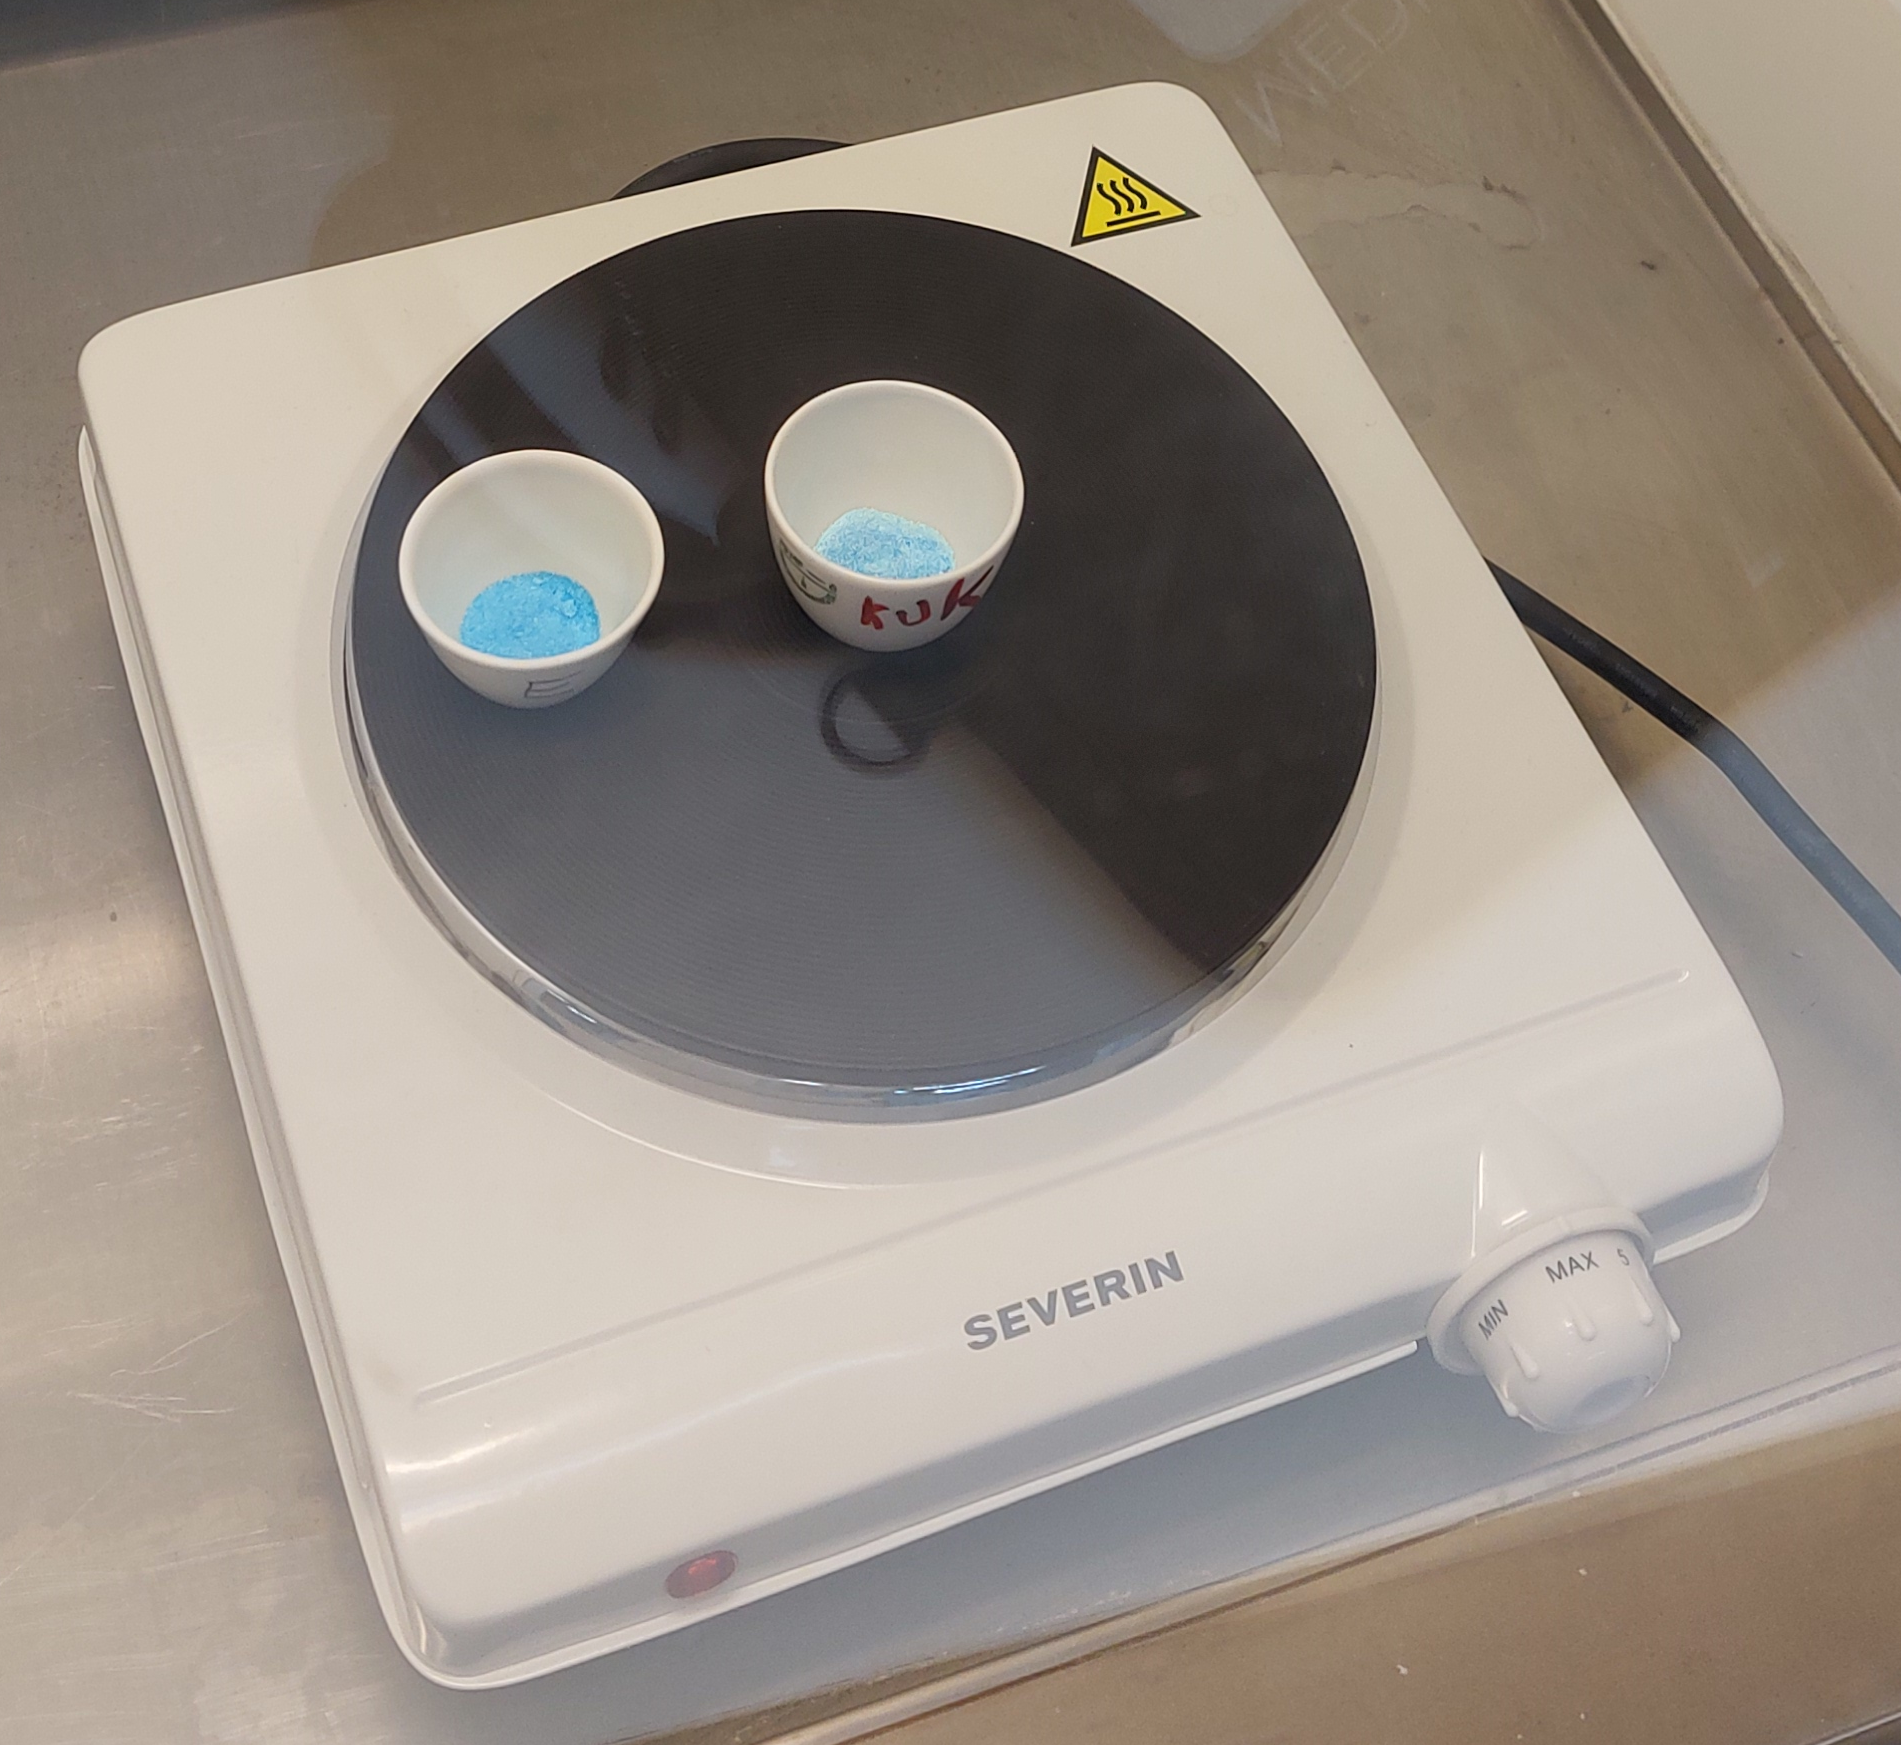
\includegraphics[width=0.9\linewidth]{plattdegel}
		\caption{Degel på värmeplatta innehållande kopparsulfat.}
		\label{fig:wrapfig}
	\end{wrapfigure}
	\begin{enumerate}
		\item En tom degel vägdes och vikten antecknades
		\item Ungefär 1 g kopparsulfat ($CuSO_4$) med kristallvatten ($H_2O$) tillsattes till degeln. Vartefter den vägdes igen (och vikten antecknades).
		\item Degeln upphettades med en kokplatta under ca 15 minuter.
		\item Degeln svalnade under ca 30 minuter, innan den vägdes igen (och vikten antecknades). 
	\end{enumerate}

	\section{Resultat}
	\subsection{Beskrivning av resultat}
	\[m_{kristalliserad-kopparsulfat}=m_{degel-med-kristalliserad-kopparsulfat}-m_{degel}\]
	\[m_{kopparsulfat-utan-kristallvatten}=m_{degel-med-kopparsulfat-utan-kristallvatten}-m_{degel}\]
	
	\pagebreak
	\section{Källförteckning}
	[1], Syntes Kemi 1 (Anders Henriksson, 2011, Gleerups) 
	\newline[ISBN: 978-91-40-67418-0]
	\newline
	
	%\bibliographystyle{apalike}
	
	%\bibliography{sample}
	
\end{document}